\section{Design And Implementation}

\subsection{Game Environments}
Tic-tac-toe and Azul provide two-player game environments that place different demands on the agents. Tic-tac-toe has a small number of legal moves, deterministic outcomes and strictly alternating turns. Azul can offer many more legal moves, while random tile draws during factory refills introduce uncertainty. During a game of Azul, turns usually alternate within a round, but the same player can make the final move of one round and the first move of the next round. These differences motivate a common set of game operations and configurations that can support both games and provide a basis for adding further environments.\\

The two environments expose a common set of operations so that agents can interact with either game. Each identifies its two players and the \texttt{current\_player}, returns the legal actions for that player using \texttt{get\_legal\_actions}, and reports whether the game has ended and who, if anyone, has won. Agents can apply a move with \texttt{make\_move}, while search agents can use \texttt{clone} to explore possible moves without changing the current game. For searches that handle randomness explicitly, \texttt{apply\_deterministic\_move} performs the predictable part of a move, \texttt{chance\_node\_required} indicates whether a random event is pending, and \texttt{resolve\_chance} performs that event where applicable. The environments also provide score bounds, a readable display, equality comparison and a game identifier for supporting tasks.\\

\begin{longtable}{@{}p{0.22\linewidth}p{0.30\linewidth}p{0.38\linewidth}@{}}
\hline
\textbf{Attribute or method} & \textbf{Purpose} & \textbf{Usage}\\
\hline
\endfirsthead

\hline
\textbf{Attribute or method} & \textbf{Purpose} & \textbf{Usage}\\
\hline
\endhead

\hline
\endfoot

\texttt{max\_\allowbreak possible\_\allowbreak score}
& Provides a score bound used to scale heuristics.
& Minimax and MCTS when configured with heuristics.\\
\hline

\texttt{min\_\allowbreak possible\_\allowbreak score}
& Declares a lower score bound to scale heuristics.
& Minimax and MCTS when configured with heuristics.\\
\hline

\texttt{player\_\allowbreak one}, \texttt{player\_\allowbreak two}
& Identify the two players.
& Minimax, MCTS and TabQL.\\
\hline

\texttt{current\_\allowbreak player}
& Identifies whose turn it is in the current state.
& Minimax, MCTS and TabQL.\\
\hline

\texttt{get\_\allowbreak legal\_\allowbreak actions()}
& Returns the legal moves available to the current player.
& Minimax, MCTS and TabQL.\\
\hline

\texttt{make\_\allowbreak move()}
& Applies a complete move, including any required random refill.
& Pure Minimax, pure MCTS and TabQL.\\
\hline

\texttt{chance\_\allowbreak node\_\allowbreak required()}
& Reports whether a random event is pending.
& Minimax and MCTS.\\
\hline

\texttt{apply\_\allowbreak deterministic\_\allowbreak move()}
& Applies the deterministic part of a move without resolving a pending random event.
& Minimax and MCTS.\\
\hline

\texttt{resolve\_\allowbreak chance()}
& Resolves a pending random event.
& Minimax and MCTS.\\
\hline

\texttt{check\_\allowbreak victory()}
& Returns the winner, or \texttt{None} if there is no winner.
& Minimax, MCTS and TabQL.\\
\hline

\texttt{check\_\allowbreak end()}
& Reports whether the game has ended, including through a draw.
& Minimax, MCTS and TabQL.\\
\hline

\texttt{clone()}
& Creates an independent game state for exploring possible continuations.
& Minimax and MCTS.\\
\hline

\texttt{display\_\allowbreak game()}
& Produces a readable representation of the game state.
& None, but used to display game to user.\\
\hline

\texttt{\_\_eq\_\_()}
& Compares game states.
& MCTS.\\
\hline

\texttt{get\_\allowbreak config()}
& Returns a string identifying the environment.
& TabQL.\\
\hline

\hline\\
\caption{Game environment attributes and methods used by the agents}
\label{tab:game-environment-interface}\\
\end{longtable}


\subsection{Minimax}

Minimax is a search-based agent that works by searching all possible game states. At the start of each decision, the player choosing a move is treated as Max and the opponent as Min. From the current game state, the agent explores each legal move and its possible successor states until the game ends. A Max win receives a favourable value, a draw receives zero, and a Min win receives an unfavourable value. These values are passed back through the tree: Max selects the highest value among its children, while Min selects the lowest. The agent then returns the move with the highest value from the current state. With tic-tac-toe, Minimax can run from the empty board in 1.16 seconds. Computing the entire game tree with Azul is estimated to take thousands of years which is why it is necessary to make changes to the pure Minimax algorithm to support Azul.

\subsubsection{Azul Compatibility (Fixed Depth Search and Chance Handling)}
As discussed in Section 4.1, Azul presents two difficulties for the full-depth Minimax agent used in tic-tac-toe: it can offer many more legal moves, and its factory refills are random. To control the cost of exploring possible moves, the fixed-depth agent searches only a specified number of moves ahead. If the game has not ended at that depth, a heuristic estimates the value of the resulting state. The Azul heuristic estimates each player’s score after resolving their current board, then compares the scores from Max’s perspective by calculating the net score difference. The graph below displays how the time taken to choose a single move increases exponentially with the search depth. \\

\begin{figure}[H]
    \centering
    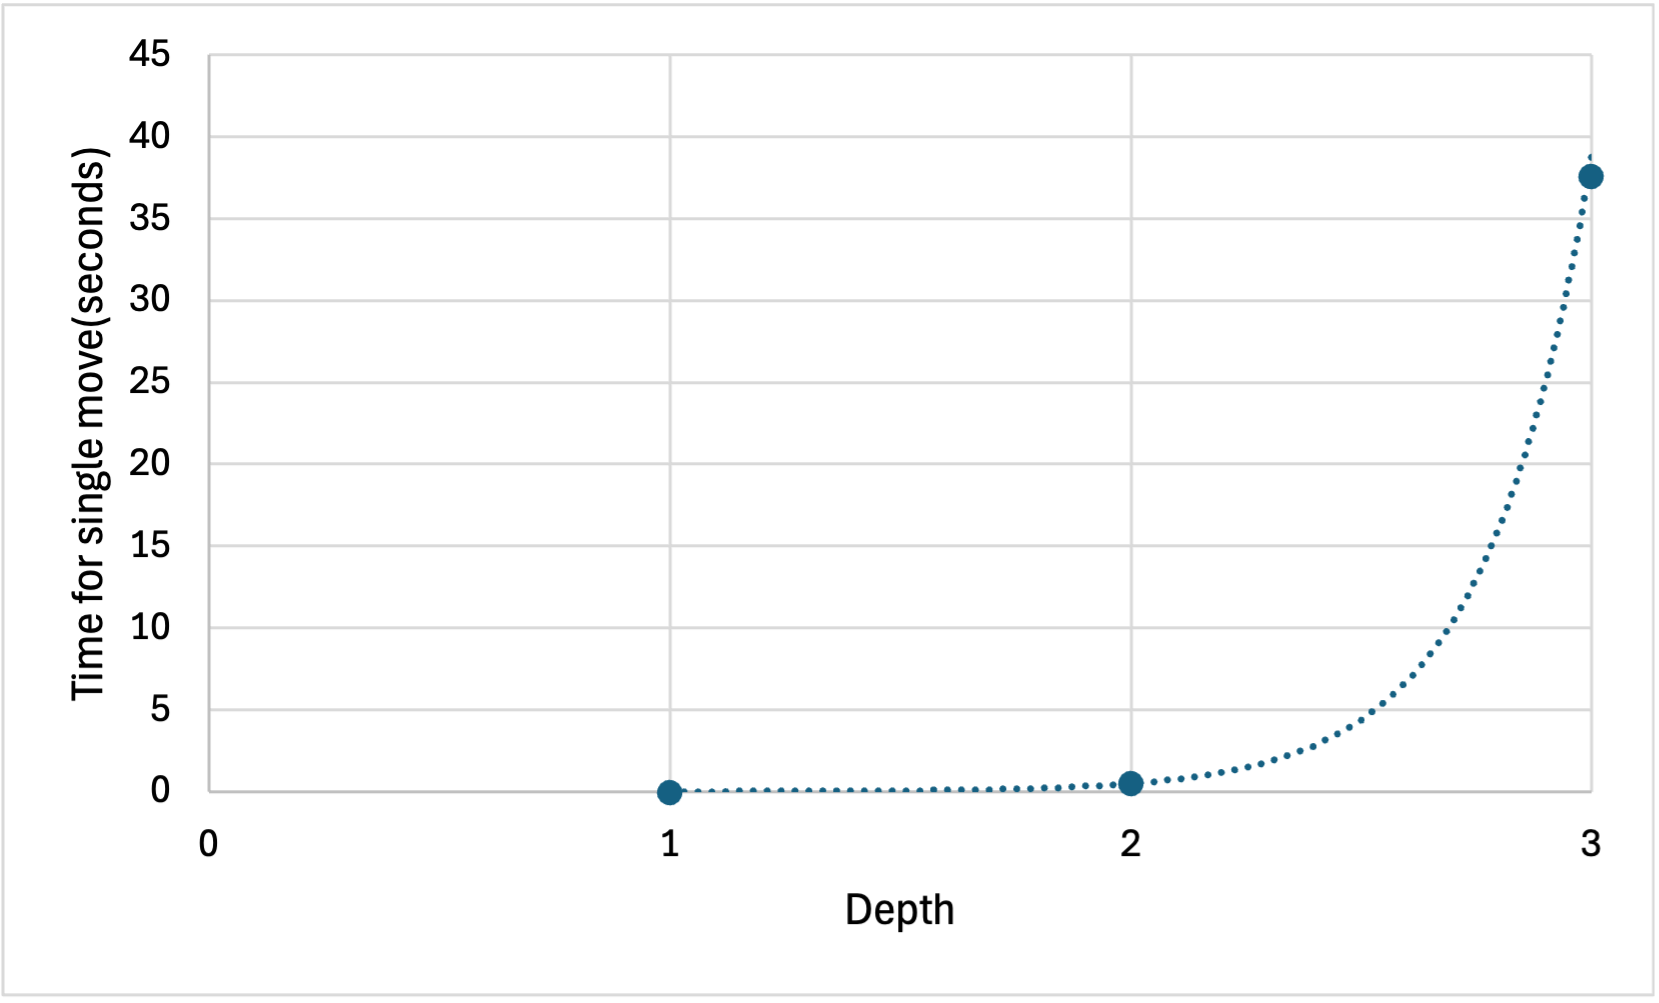
\includegraphics[width=0.7\textwidth]{report/graphs/fixed-depth-minimax-depth-runtime.png}
    \caption{Minimax decision time at different search depths in Azul.}
    \label{fig:minimax-runtime-depth}
\end{figure}

The random refills require a separate decision about how the search should continue. The fixed-depth agent therefore uses a configurable chance policy when a refill is needed. The round termination policy stops the search at that point and evaluates the state with the heuristic. The sampled refills policy generates a specified number of possible refills, continues the search from each resulting state, and averages their values. The graph below shows a comparison between net score and full game runtime across different number of samples. \\

\begin{figure}[H]
    \centering
    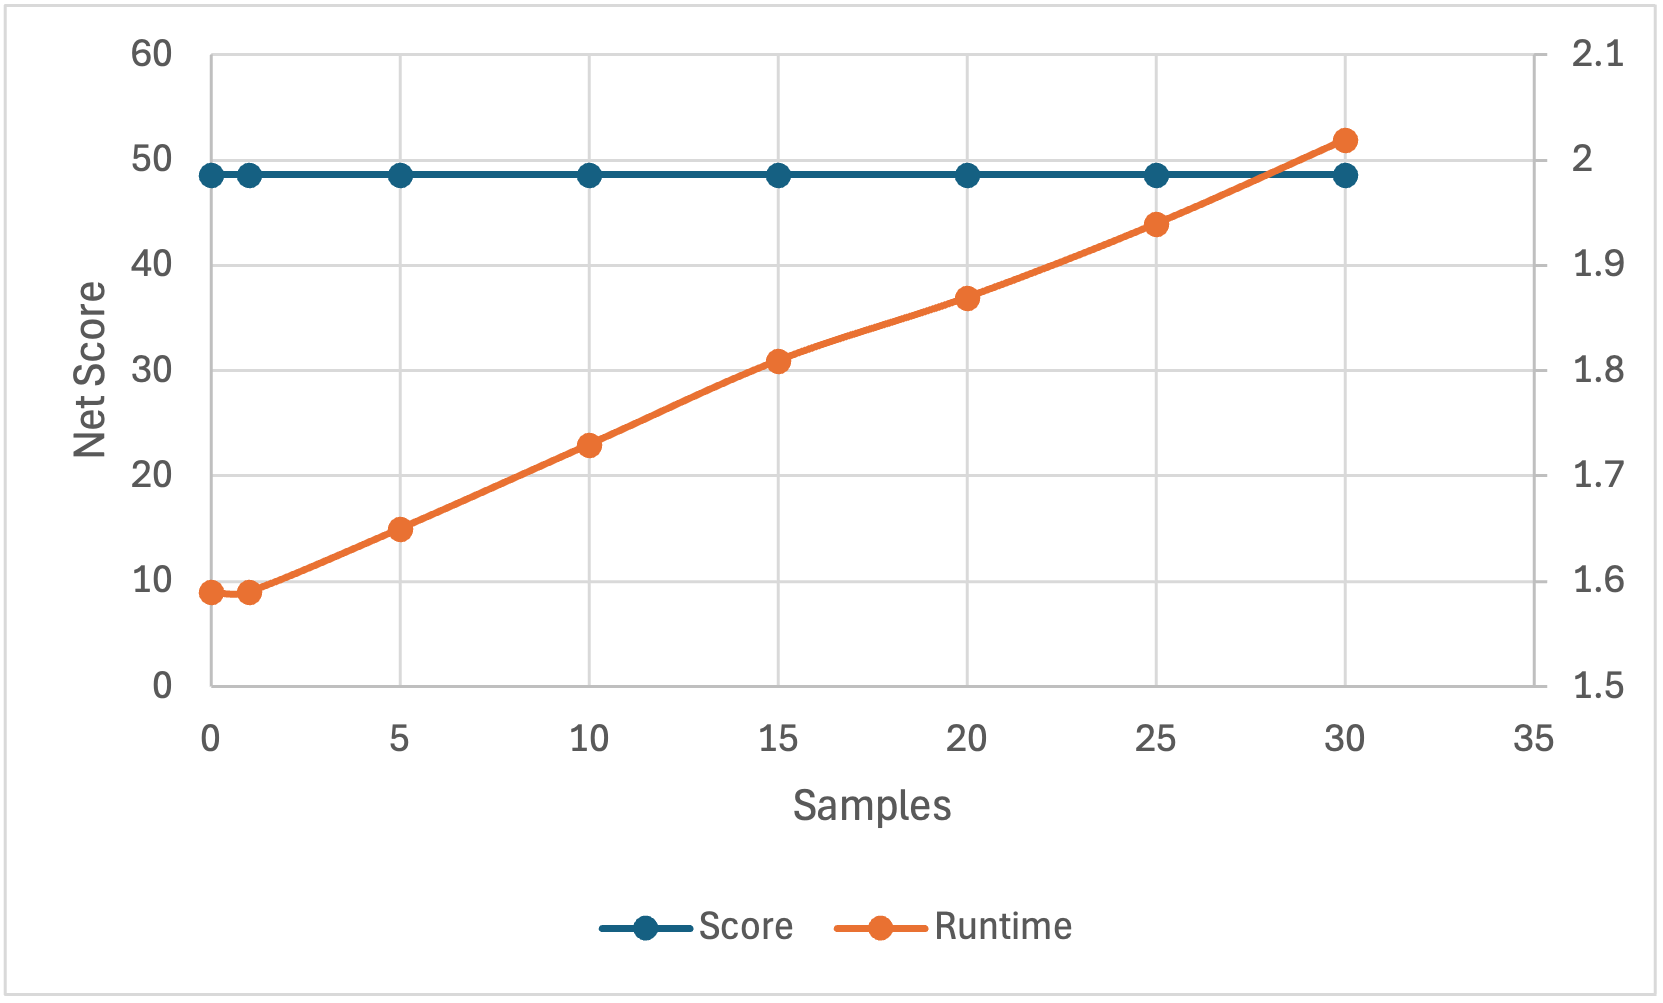
\includegraphics[width=0.85\textwidth]{report/graphs/fixed-depth-minimax-chance-policy.png}
    \caption{Minimax game time and net score using different numbers of samples.}
    \label{fig:minimax-chance-policy}
\end{figure}

Although the net score does not improve with the increase in number of samples, this is highly likely due to the search depth being 2. Using the sampled refills policy with 5 samples appears to provide a good trade-of between time and the ability to reason about the outcomes of a random refill. Running fixed-depth Minimax at a max depth of 3, with 5 sampled refills results in an average net score of 54.2 and an average full-game runtime of 78.09 seconds.